\section{Proposed Methods}


\subsection{Toxicity Detection with KNNs}

This approach is based on the few-shot prompting method for classification.
Few-shot prompting means we provide the model with some examples for the task it is being trained on.
This is a powerful tool used with transformer models to improve their performance significantly.
Research has shown that transformers can utilize their pre-trained knowledge more efficiently when provided with some examples in the prompt.

The downside of few-shot prompting is that the user has to manually add a relevant example in the prompt.
Our approach automates this task to detect toxic content.
We utilize vector databases to find similar toxic and benign examples for a given text.
Moreover, the database is also updated with the latest texts the model identifies during inference, which means the model updates its memory each time it sees a new text.

A vector database stores vector representation of unstructured data.
We have an option to "query" the database with a given vector to find its nearest neighbours or similar vectors.
The vector embeddings for text and image data are formed using encoder-only transformer models.
We use Pinecone as our vector database.

We experiment with different numbers of examples to be extracted from the database and report our results in \autoref{tab:results}.
Below table contains the probabilities of toxicity in text

\begin{table}[h!]
\centering
\begin{tabular}{|c|c|c|c|}
\hline
{\textbf{text}} & \multicolumn{3}{c|}{\textbf{k-shot prompting}} \\ \cline{2-4} 
& \textbf{0 - shot} & \textbf{2 - shot} & \textbf{4 - shot} \\ \hline
I will stab you in the back& 0.99648 & 0.99969 & 0.99972\\ \hline
I will kill animals& 0.98987 & 0.99955 & 0.99970 \\ \hline
you can suck my ... & 0.99685 & 0.99934 & 0.99948 \\ \hline
\end{tabular}
\caption{Toxicity with k-shot prompting}
\label{tab:results}
\end{table}
We can see our approach of k-shot prompting helps us detect the toxicity better.


\subsection{Toxicity-Attended Roberta Classification}

\subsubsection{Motivation}
Detecting offensive or toxic language on social media is a challenging task, as context plays a crucial role in determining whether a statement is harmful or benign. Consider the following examples:
\begin{enumerate}
    \item (Toxic): "You are a fucking idiot."
    \item (Non-Toxic): "That movie was so fucking amazing."
\end{enumerate}
Although both sentences contain the same profane word, their toxicity differs based on context. The first statement is clearly an insult, while the second is an expression of enthusiasm. This highlights the importance of analyzing the context surrounding profane words to accurately classify language as toxic or non-toxic. But on professional platforms like LinkedIn, the same examples should be flagged as toxic due to the professional setting.
Existing models are designed to detect offensive content but often lack a targeted mechanism to capture the nuanced context of profane or offensive words. To address this limitation, we propose the Toxicity-Attended Roberta Classification, a modified version of the \textit{unitary/unbiased-toxic-roberta} model designed to improve the sensitivity and accuracy of toxicity detection.

\subsubsection{Key Contributions}
\begin{itemize}
    \item \textbf{Context-Aware Attention:} An additional attention mechanism tailored to focus on profane words and their surrounding context.
    \item \textbf{Curated Profanity Queries}: Leveraging a list of profane words sourced from CMU as the queries in the custom attention layer.
    \item \textbf{Enhanced Representation:} By selectively attending to offensive language patterns, the model gains deeper insights into the context, thereby improving its performance.
\end{itemize}

\subsubsection{Proposed Approach}
Our architecture builds upon the \textit{unitary/unbiased-toxic-roberta} model with the following modifications:
\begin{enumerate}
    \item \textbf{Toxicity-Attended Attention Block:}
    \begin{itemize}
        \item \textbf{Queries:} A curated list of profane words (e.g., \textit{"idiot," "fucking," "stupid,"} etc.).
        \item \textbf{Keys \& Values:} Derived from the embeddings of the input text.
    \end{itemize}
    This additional attention block uses profane words as queries to focus on the regions of the input text that are most relevant to determining toxicity. The block selectively amplifies the context surrounding these words, allowing the model to make informed predictions.
    
    \item \textbf{Contextual Analysis via Attention:}  
    Attention mechanisms excel at identifying relevant parts of the input for a given task. By passing swear words as queries, the model ensures that its focus remains on the parts of the input that may signal offensive language, even when it is expressed subtly or ambiguously.
\end{enumerate}

\subsubsection{Examples and Insights}
The proposed approach improves the model’s ability to handle nuanced cases, as shown below:

\begin{enumerate}
    \item \textbf{Ambiguous Profanity:}
    \begin{itemize}
        \item \textbf{Input:} "This game is so fucking bad!"\\
        \textbf{Context:} Indicates dissatisfaction with the game (toxic).
        \item \textbf{Input:} "This party is so fucking good!"\\
        \textbf{Context:} Indicates enthusiasm about the party (non-toxic).
    \end{itemize}
    By analyzing the context around the toxic words, the model distinguishes between toxic and non-toxic usages of profanity.
    
    \item \textbf{Professional Context:}  
    In platforms like LinkedIn, the same examples should be flagged as toxic due to the professional setting. Our model’s architecture can be adapted for such domain-specific requirements by tailoring the queries or modifying the threshold for toxicity classification.
\end{enumerate}

\subsubsection{Architecture}
Figure \ref{fig:models-diff} compares the original and modified architectures:

\begin{itemize}
    \item \textbf{Baseline (unitary/unbiased-toxic-roberta):} Standard encoder blocks with self-attention for general contextual representation.
    \item \textbf{Enhanced Model:} Includes an additional Toxicity-Attended Attention Block, which explicitly focuses on offensive content. This block can be operated in parallel with the original self-attention layers, enabling a faster inference while maintaining context awareness.
\end{itemize}

\subsubsection{Benefits of the Proposed Approach}
\begin{enumerate}
    \item \textbf{Improved Sensitivity:} By explicitly attending to profane words, the model captures subtle shifts in meaning caused by context.
    \item \textbf{Domain Adaptability:} The query list can be modified to suit different domains, such as social media, professional platforms, or gaming communities.
    \item \textbf{Robustness to Ambiguity:} Handles cases where offensive language may appear non-toxic or vice versa.

    \begin{table}[!ht]
    \centering
    \begin{tabular}{c|c|c|c}
        \hline
        \textbf{Model} & \textbf{Toxigen} & \textbf{SBIC} & \textbf{DHate} \\
        \hline
        ChatGPT-DToT+FS+R & \textbf{87.03} & 72.00 & 69.20 \\
        ChatGPT-DToT+FS & 86.03 & 71.70 & 69.50 \\
        \hline
        RoBerta & 82.10 & 85.50 & 87.30 \\
        RoBerta-kNNs & 82.50 & \textbf{86.27} & \textbf{89.20} \\
         \hline
    \end{tabular}
    \caption{Accuracy scores on datasets}
    \label{tab:my_label}
    \end{table}

    \begin{table}[h!]
    \centering
    \begin{tabular}{l c}
    \toprule
    \textbf{Model} & \textbf{F1-score} \\
    \midrule
    Generative Cls+demo & 0.60 \\
    RoBerta + kNNs & \textbf{0.79} \\
    \bottomrule
    \end{tabular}
    \caption{Comparison of Models and Their F1-scores.}
    \label{tab:model_f1}
    \end{table}
    
\end{enumerate}

\begin{figure*}[t] 
    \centering
    \begin{subfigure}[h]{0.47\linewidth} 
        \centering
        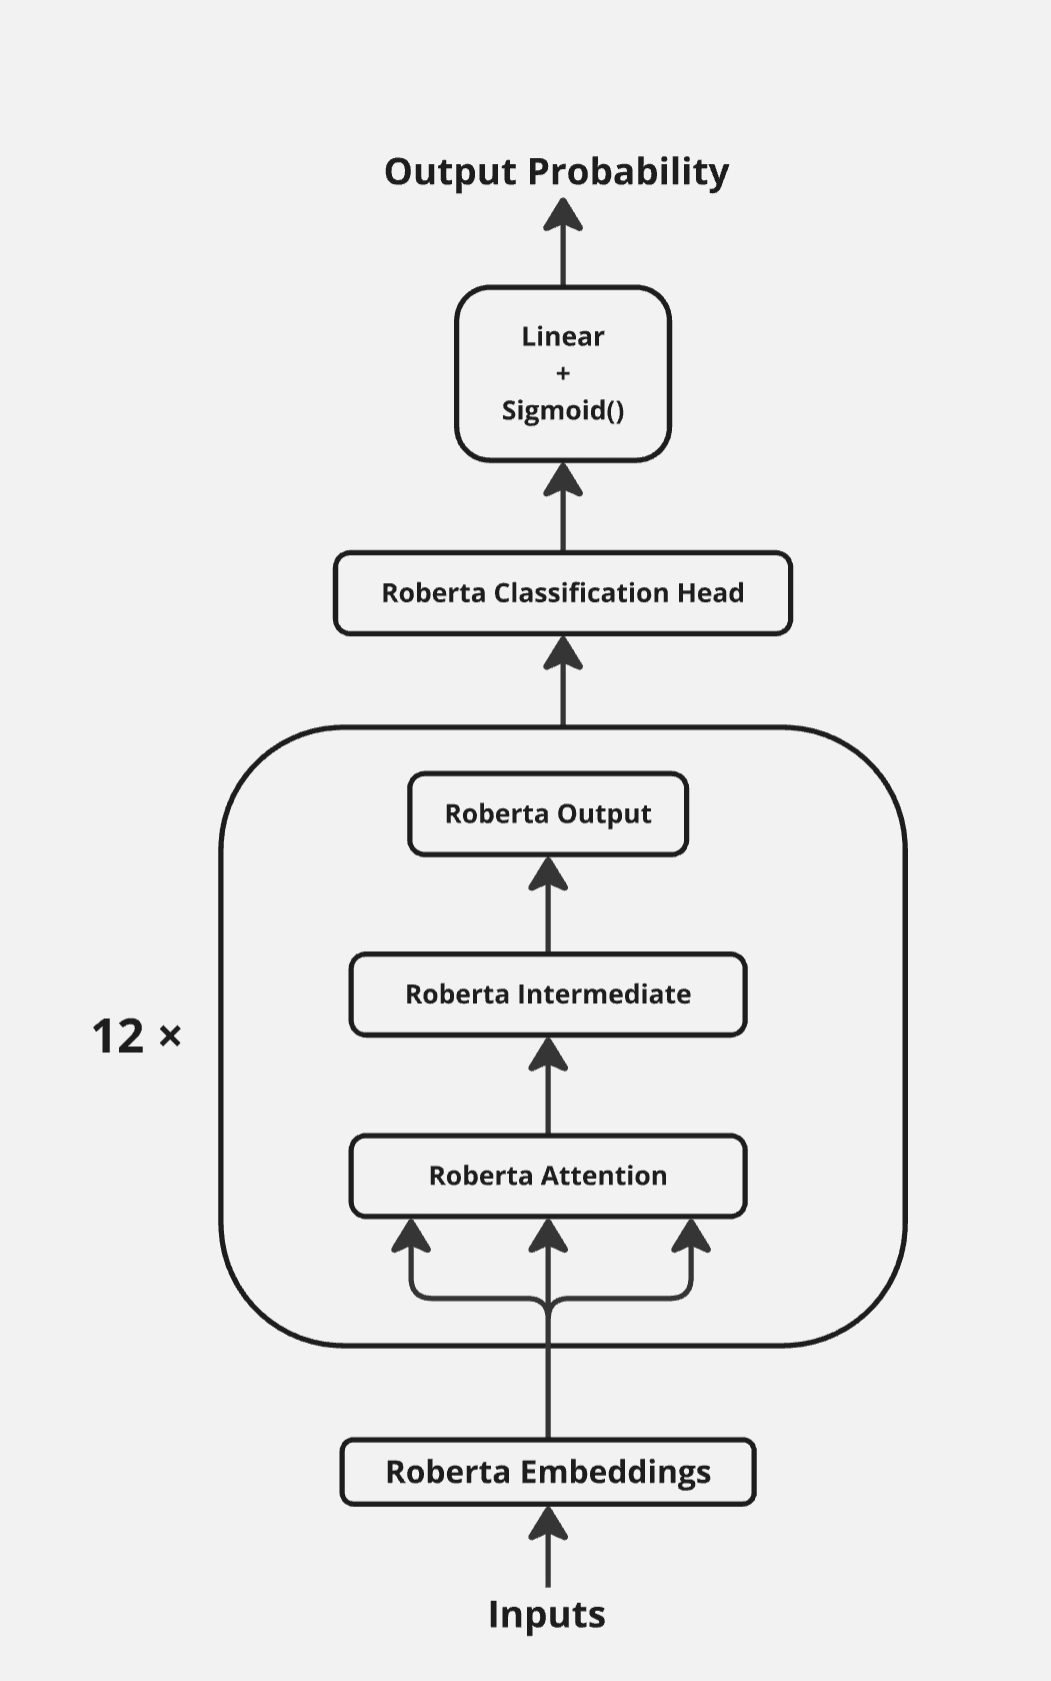
\includegraphics[width=\linewidth]{Images/Screenshot_20241023_113542_Miro.jpg}
        \caption{Original unitary/unbiased-toxic-roberta model}
        \label{fig:org-model}
    \end{subfigure}
    \hspace{0.02\linewidth} % Small space between subfigures
    \begin{subfigure}[h]{0.47\linewidth} 
        \centering
        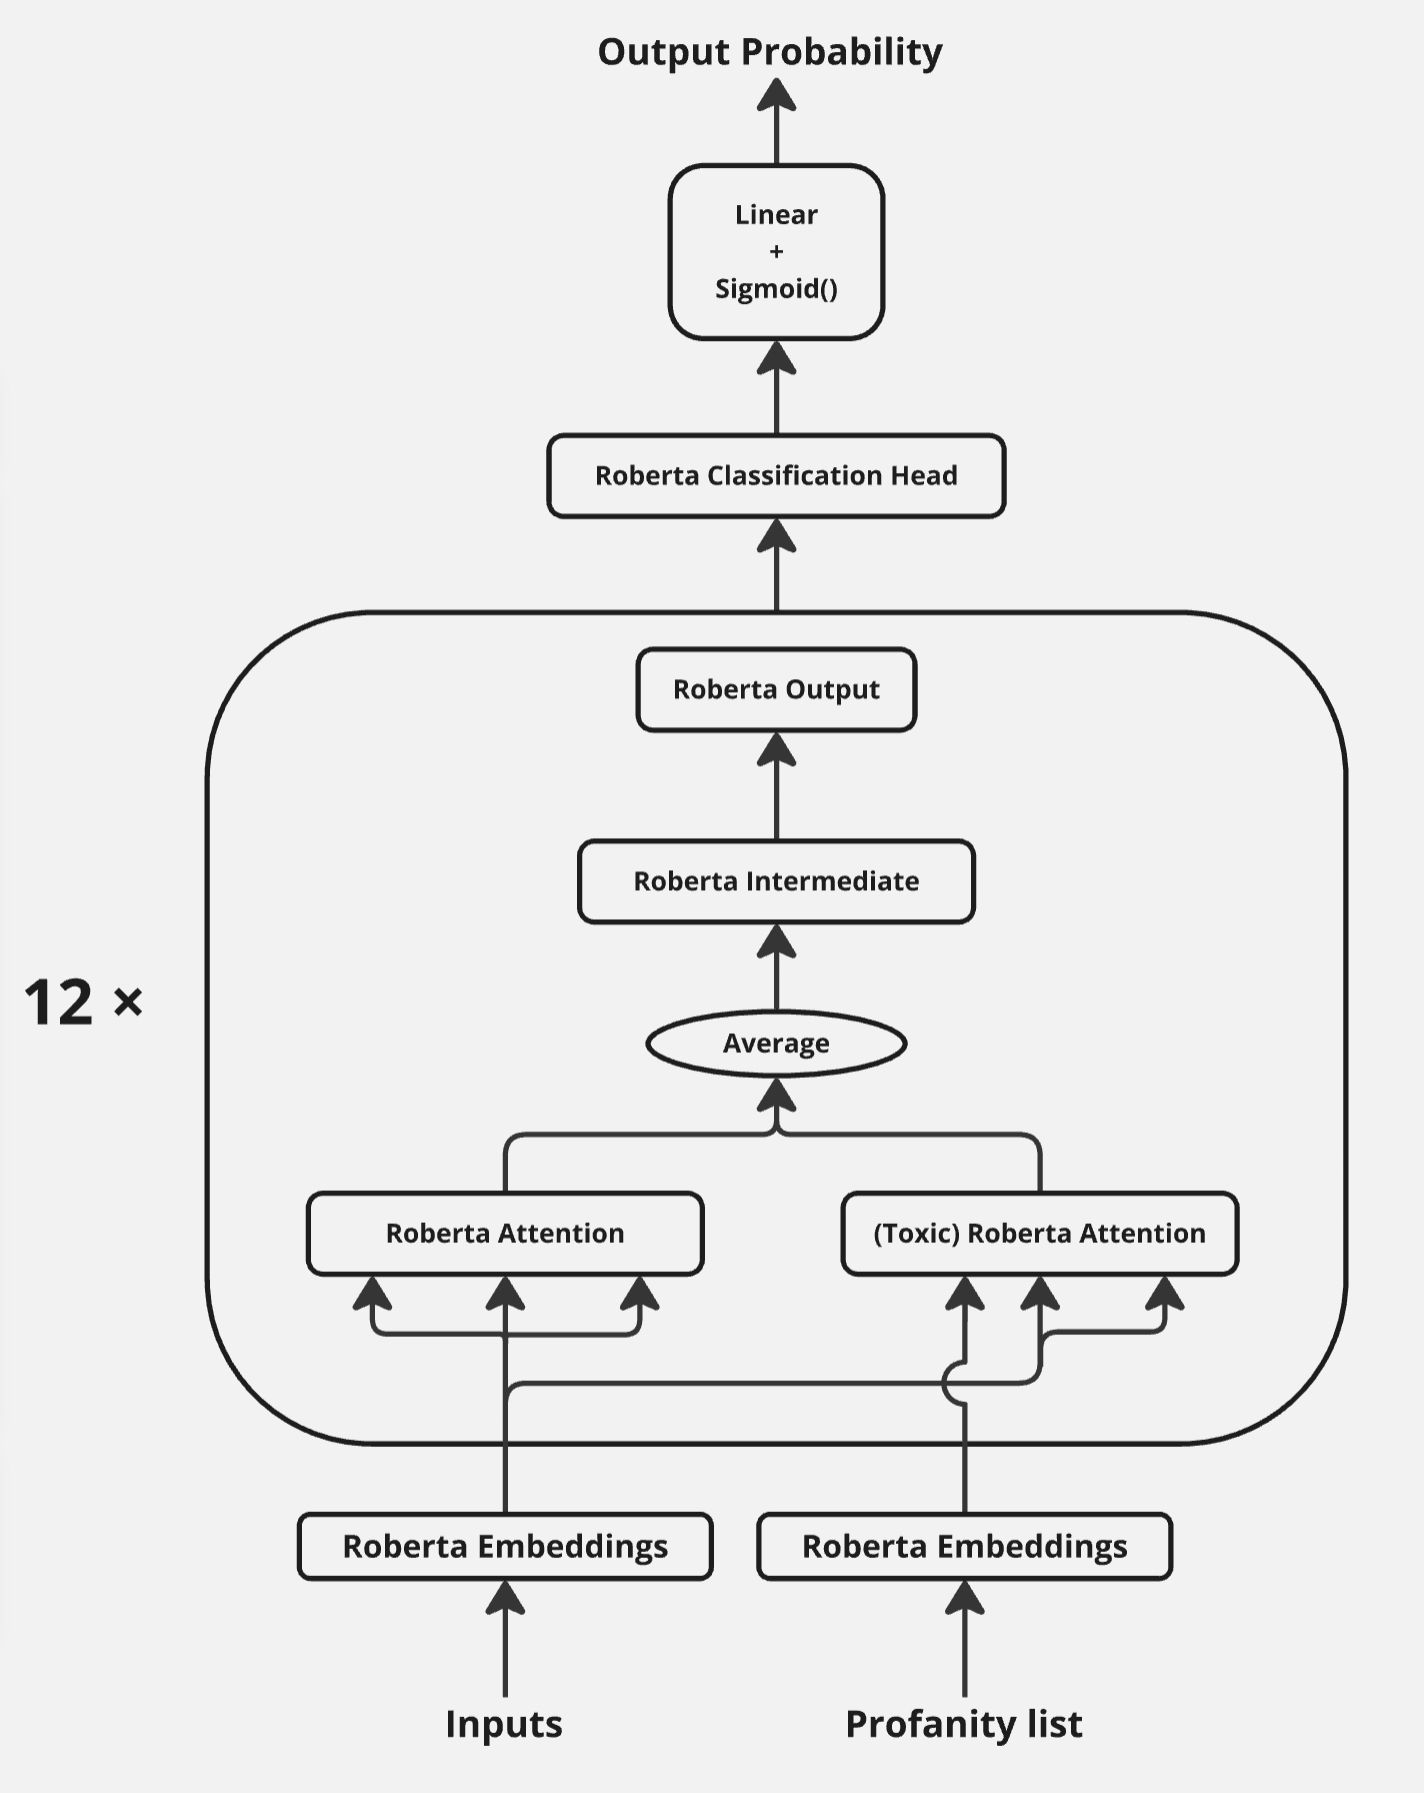
\includegraphics[width=\linewidth]{Images/Screenshot_20241023_113521_Miro.jpg}
        \caption{Toxic-attended roberta model}
        \label{fig:modified-model}
    \end{subfigure}
    \caption{Comparison between the original unitary/unbiased-toxic-roberta model and the modified Toxic-attended Roberta model}
    \label{fig:models-diff}
\end{figure*}




